\chapter{Impl\'ementation de la solution}

\section{Introduction}

Ce chapitre aborde comme sujet les choix technologiques et les outils pour l'impl\'ementation de notre solution ainsi que les captures d'\'ecran des diff\'erents fen\^etre r\'ealiser et les tests de validation effectu\'es sur les modules d\'evelopp\'es.

\section{Environnement logiciel}
L'environnement logiciel utilis\'e pour la r\'ealisation de notre projet est pr\'esent\'e dans le tableau suivant :

\begin{table}[H]
\begin{center}
\begin{tabularx}{\textwidth}{ |l|X| }
\hline Outil & Description \\\hline \hline
JDK 1.8 & Java Development Kit (JDK) d\'esigne un ensemble de biblioth\`eques logicielles de base du langage de programmation Java.\\ \hline
Intellij IDEA & Environnement de d\'eveloppement int\'egr\'e (IDE).\\ \hline
Visual Studio Code & Environnement de d\'eveloppement c\^ote frontend.\\ \hline
Android Studio & Environnement de d\'eveloppement pour d\'evelopper des applications mobiles Android.\\ \hline
GitBash & C'est une ligne de commande dans laquelle on peut ex\'ecuter les commandes git.\\ \hline
Zeplin & C'est un outil de design des fonctionnalit\'es. Permet de collaborer entre les designers et les d\'eveloppeurs frontends, facile, efficace et permet de gagner du temps.\\ \hline
Postman & Est actuellement l'un des outils les plus populaires utilis\'es dans les tests d'\gls{API}.\\
\hline
\end{tabularx}
\caption{Environnement logiciel}
\end{center}
\end{table}

\section{Architecture technique du syst\`eme}

Notre syst\`eme se base en totalit\'e sur l'architecture orient\'e service et plus pr\'ecis\'ement sur l'architecture \gls{REST}. C'est un style d'architecture pour la conception d'applications faiblement coupl\'ees sur \gls{HTTP}, souvent utilis\'e dans le d\'eveloppement de services Web.

Une \'etude qui a \'et\'e faite par l'entit\'e \gls{DF}, ils sont convaincu d'adapter quelques technologies \& outils dans tous les projets. La figure suivante repr\'esente les technologies \& les biblioth\`eques essentiels utilises dans notre projet.

\begin{figure}[H]
	\center{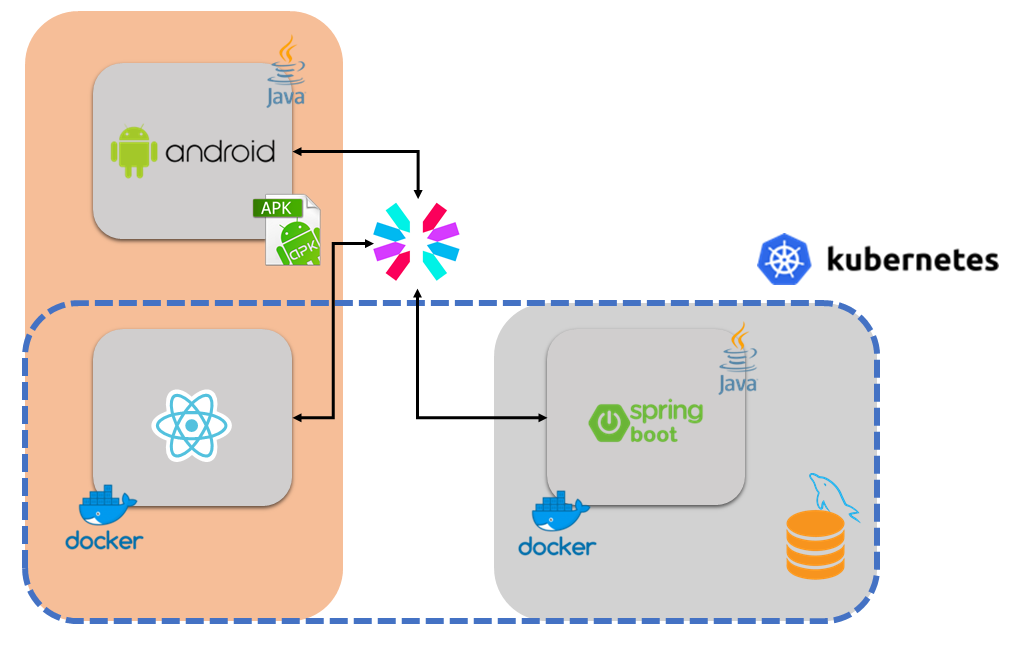
\includegraphics[width=\textwidth]{Figures/achitec-tech.PNG}}
	\caption{\label{fig:my-label} Architecture technique du syst\`eme}
\end{figure}

Maintenant, on va expliquer l'utilit\'e des technologies utilises dans notre impl\'ementation. 

\subsection{Couche BackEnd}
\begin{itemize}

\item \textcolor{spring}{SpringBoot} : est un framework Java open source utilis\'e pour cr\'eer un Micro Service. Il est d\'evelopp\'e par l'\'equipe \textbf{pivotal}. Il est facile de cr\'eer des stand-alone applications. Spring Boot contient une prise en charge compl\`ete de l'infrastructure pour le d\'eveloppement d'un micro-service et vous permet de d\'evelopper des applications d'entreprise.

\item \textbf{Spring Security} : est un Framework de s\'ecurit\'e l\'eger qui fournit une authentification et un support d'autorisation afin de s\'ecuriser les applications Spring. Il est livr\'e avec des impl\'ementations d'algorithmes de s\'ecurit\'e populaires.

\item \textbf{Swagger} : nous permet de d\'ecrire la structure de nos API afin que les machines puissent les lire. La capacit\'e des API \`a d\'ecrire leur propre structure facilite aux d\'eveloppeurs frontend la communication avec nos serveurs.

\item \gls{JWT} : est une normalisation permettant d'utiliser des jetons pour s'authentifier sur le Web en g\'en\'eral. Il est robuste et peut contenir beaucoup d'informations. Comme tout autre jeton, JWT peut \^etre utilis\'e pour transmettre l'identit\'e d'utilisateurs authentifi\'es entre un fournisseur d'identit\'e et un fournisseur de services. Il peut \'egalement contenir toutes les revendications de l'utilisateur, telles que les donn\'ees d'autorisation. Le fournisseur de services n'a donc pas besoin d'entrer dans la base de donn\'ees ou dans des syst\`emes externes pour v\'erifier les r\^oles et autorisations des utilisateurs pour chaque demande. Ces donn\'ees sont extraites du jeton.

\end{itemize}

\subsection{Couche FrontEnd}

On a suivre \textbf{Material Design} dans toutes les interfaces de notre application (est un ensemble de r\`egles de design propos\'ees par \textbf{Google} et qui s'appliquent \`a l'interface graphique des logiciels et applications).

Cette couche d\'ecompose \`a deux parties :

\subsubsection{Couche FrontOffice}

Pour la partie frontOffice, on a une application mobile d\'evelopp\'e par android native, utilisant le langage JAVA pour une tablette sp\'ecifique utiliser dans les chantiers du groupe \gls{OCP}. 

\subsubsection{Couche BackOffice}
\begin{itemize}

\item \textcolor{react}{ReactJS} : est essentiellement une biblioth\`eque JavaScript open-source qui est utilis\'ee pour cr\'eer des interfaces utilisateur sp\'ecifiquement pour les applications \`a page unique. React nous permet \'egalement de cr\'eer des composants d'interface utilisateur r\'eutilisables.

\item \textcolor{redux}{Redux} : Biblioth\`eque compl\'ementaire \`a React qui permet de conserver facilement les donn\'ees (State) et les \'ev\'enements (Actions) .Redux isole l'objet d'\'etat des composants.

\item \textbf{Redux-saga} : est une biblioth\`eque de middleware redux con\c{c}ue pour simplifier la gestion des effets secondaires de votre application redux. Pour ce faire, il exploite une fonctionnalit\'e de l'ES6 appel\'ee Generators, qui nous permet d'\'ecrire un code asynchrone qui a l'air synchrone et qui est tr\`es facile \`a tester.

\end{itemize}

\subsection{Couche Base de donn\'ees}
\begin{itemize}
\item \textbf{MySQL} : est un syst\`eme de gestion de base de donn\'ees relationnelle open source bas\'e sur le langage \gls{SQL}. Leur utilit\'e est faire stocker les donn\'ees textuel de notre application.
\item \textbf{MINIO} : est un serveur de stockage d'objets haute performance compatible avec les API Amazon S3. Pour faire stocker les attachements de l'application ( images \& audios ).
\end{itemize}

\subsection{Outils de DevOps}

\begin{itemize}
\item \textbf{Docker} : est un outil con\c{c}u pour faciliter la cr\'eation, le d\'eploiement et l'ex\'ecution d'applications \`a l'aide de conteneurs. Les conteneurs permettent \`a un d\'eveloppeur de conditionner une application avec toutes les pi\`eces dont il a besoin, telles que des biblioth\`eques et autres d\'ependances, et de l'exp\'edier dans un package unique.

\item \textbf{Kubernetes} : est un syst\`eme d'orchestration de conteneur open-source permettant d'automatiser le d\'eploiement, la mise \`a l'\'echelle et la gestion des applications.

\end{itemize}

\section{Impl\'ementation \& tests}

Nous avons r\'eparti le travail en plusieurs it\'erations (Sprints). Le sprint est un bloc de temps (1 semaine) durant lequel un incr\'ement du produit sera r\'ealis\'e. Tous les sprints ont le m\^eme dur\'ee et ne chevauchent jamais. Tout au long de cette partie, on va traiter le sprint 5 "Cr\'eer un chantier" comme mod\`ele pour tous les autres sprints, puis on va donner des captures d'\'ecran de la r\'esultat courant du notre projet avec les tests de validation.

\subsection{Sprint mod\`ele : Cr\'eer un chantier}

\subsubsection{Description g\'en\'erale du sprint}

Au cours de ce sprint nous sommes focalis\'es sur la cr\'eation d'un chantier. Dans un premier temps, on va afficher une \'ecran qui permet au utilisateur de remplir les \'el\'ements n\'ecessaire pour cr\'eer un chantier. Cette sprint se base sur la partie frontOffice (concernant l'utilisateur de l'application mobile).

\subsubsection{Description d\'etaille du sprint}

Apr\`es l'authentification, le prospecteur passe \`a l'\'ecran d'accueil. Puis, l'application peut suivre les d\'emarches suivantes :
\begin{figure}[H]
	\center{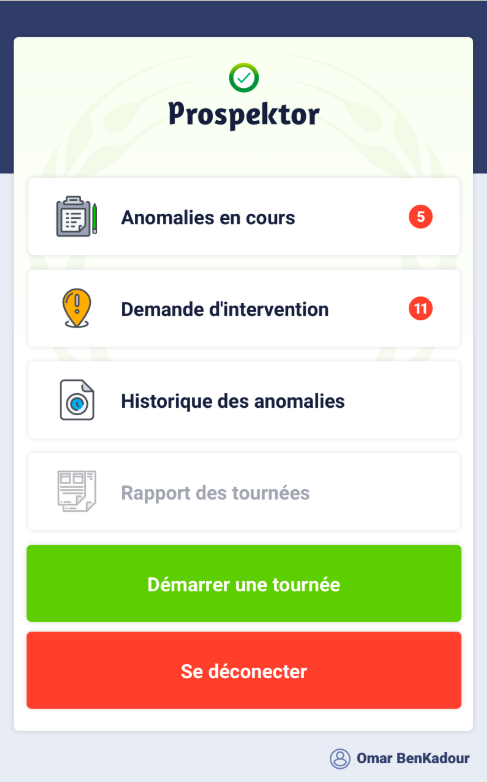
\includegraphics[width=0.4\textwidth]{Figures/acceuil.PNG}}
	\caption{\label{fig:my-label} Ecran d'acceuil}
\end{figure}
\begin{itemize}
\item Prospecteur peut cliquer sur le button (D\'emarrer une tourn\'ee).
\item la tablette envoie au serveur une requ\^ete pour g\'en\'erer un chantier vide et recevoir leur identifiant.
\item Passant \`a l'autre \'ecran qui contient les d\'etails d'un chantier.
\item Avant afficher l'\'ecran, la tablette demande au serveur toutes les informations sur les machines, zones, trench\'ees \& sorties d'une mine sp\'ecifique.
\item Apr\'es la r\'eception de ces informations, l'\'ecran sera afficher et le prospecteur peut remplir les champs de chantier d'une fa\c{c}on ordonn\'ee.
\begin{figure}[H]
	\center{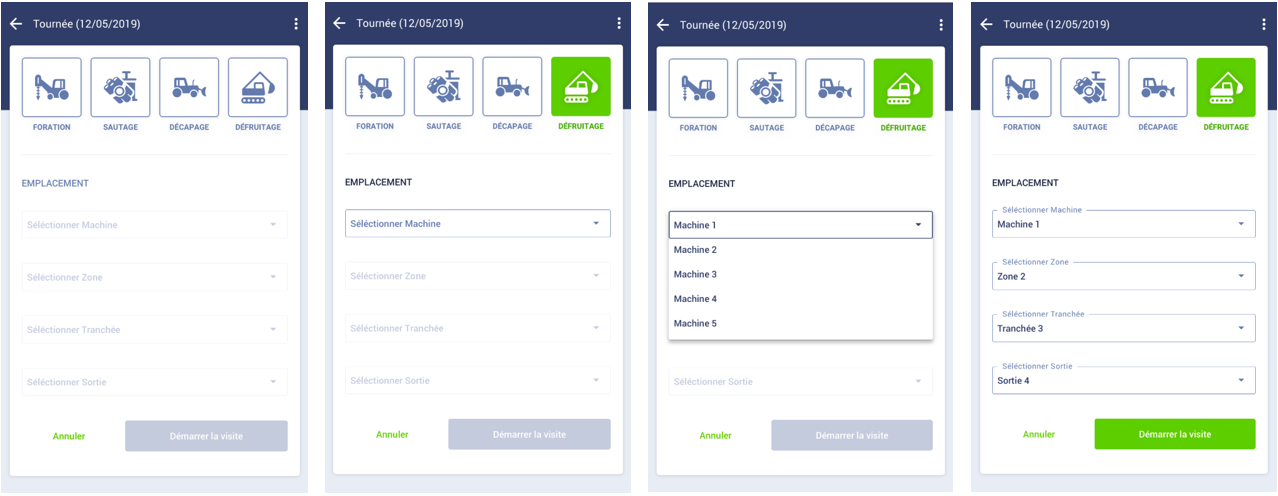
\includegraphics[width=\textwidth]{Figures/chantier.PNG}}
	\caption{\label{fig:my-label} \'Ecran de chantier}
\end{figure}
\item Enfin, une button pour la  confirmation.
\item une requ\^ete sera envoy\'e au serveur qui contient tout les informations sur cette tourn\'ee.
\end{itemize} 

On a d\'eveloppe les derni\`eres \'ecran par android studio. respectant l'architecture \gls{MVP} qu'on a d\'ej\`a expliq\'e.

\begin{figure}[H]
	\center{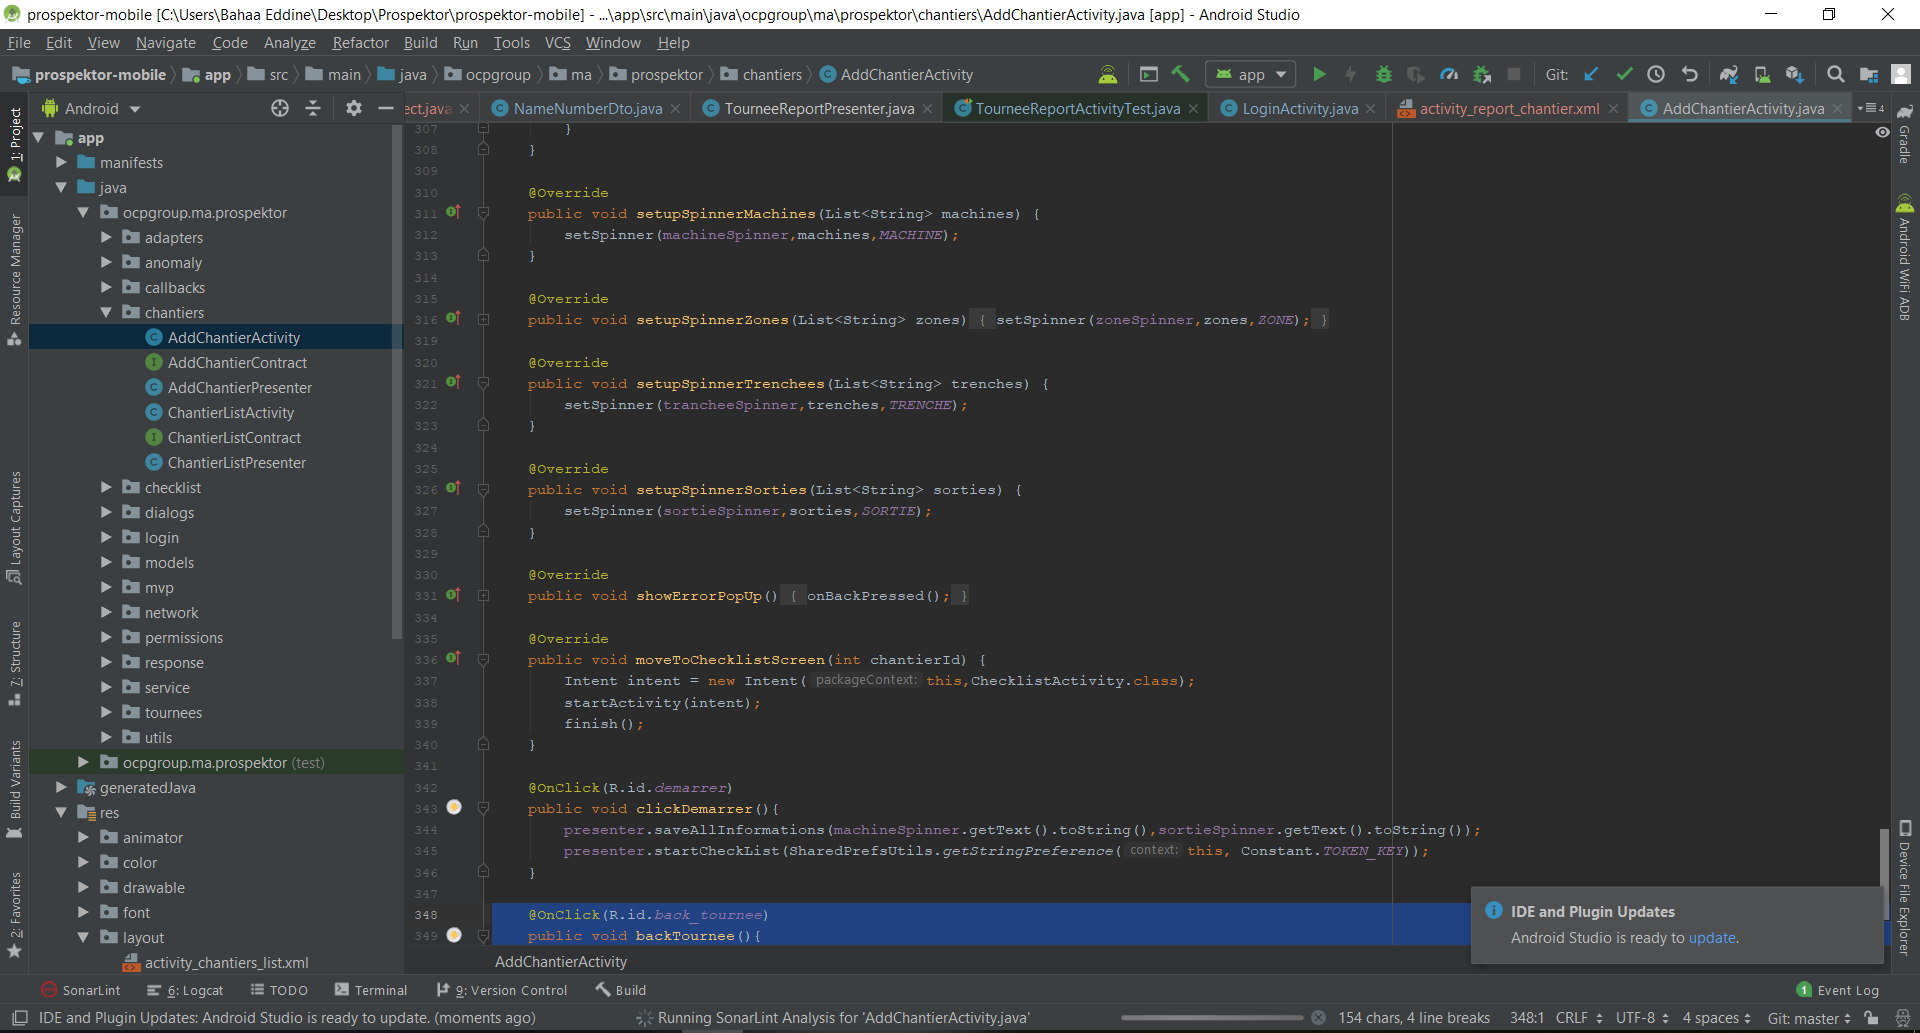
\includegraphics[width=\textwidth]{Figures/androidstudio.PNG}}
	\caption{\label{fig:my-label} Outil Android Studio}
\end{figure}

\subsection{Captures d'\'ecran du r\'esultat courant}

Pour la r\'esultat courant de notre application. On a cr\'ee les proc\'edures suivantes : 

\subsubsection{Prospecteur WorkFlow}

ce qui concerne le frontoffice pour l'utilisateur prospecteur, il peut suivre les \'etapes suivantes :

\begin{figure}[H]
	\center{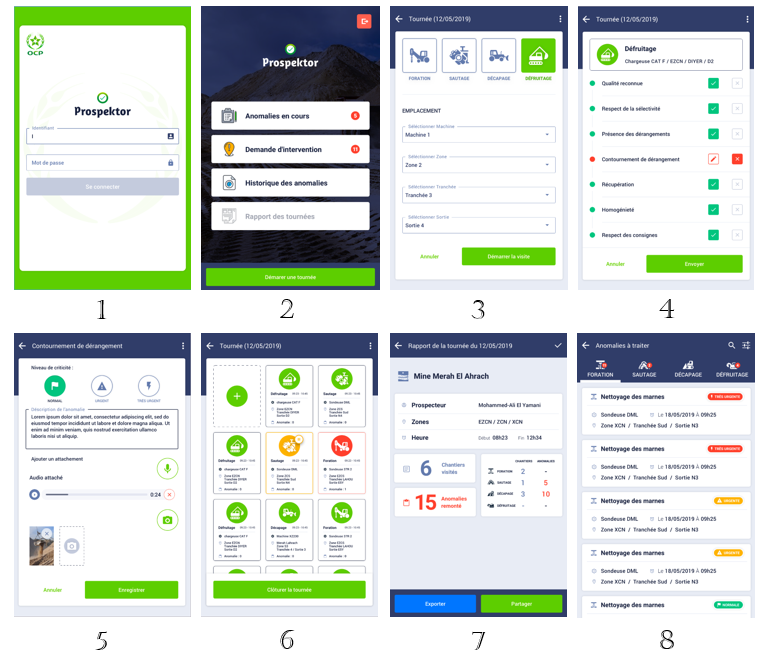
\includegraphics[width=\textwidth]{Figures/workflowprospector.PNG}}
	\caption{\label{fig:my-label} Prospecteur WorkFlow}
\end{figure}

\textbf{1} : Authentification

\textbf{2} : Page d'accueil

\textbf{3} : Cr\'eation d'un chantier

\textbf{4} : Checklist d'un chantier

\textbf{5} : Creation d'une anomalie \& Ajouter des attachements

\textbf{6} : liste des chantiers

\textbf{7} : Rapport d'une tour\'ee

\textbf{8} : liste des anomalies

\subsubsection{Exploitant WorkFlow}

ce qui concerne le frontoffice pour l'utilisateur exploitant, il peut suivre les \'etapes suivantes :

\begin{figure}[H]
	\center{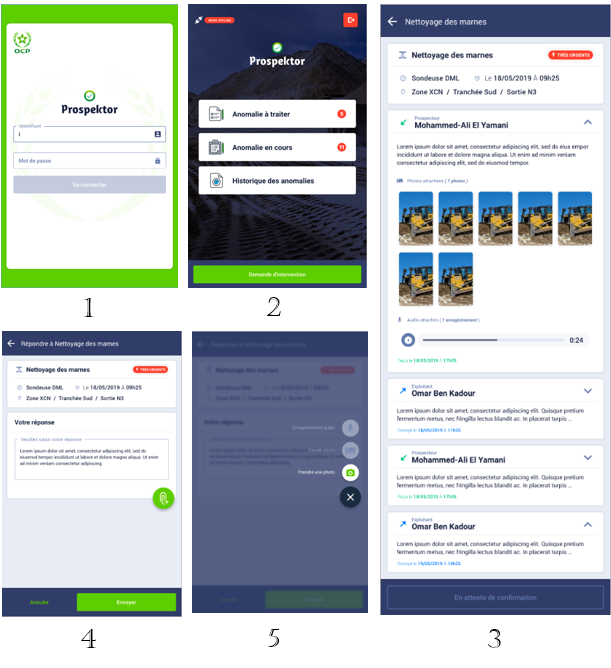
\includegraphics[width=\textwidth]{Figures/workflowexploitant.PNG}}
	\caption{\label{fig:my-label} Exploitant WorkFlow}
\end{figure}

\textbf{1} : Authentification

\textbf{2} : Page d'accueil

\textbf{3} : liste des anomalies cr\'eer par les prospecteurs

\textbf{4,5} : Creation d'une anomalie \& Ajouter des attachements


\subsection{Test de validation}

\section{Conclusion}





